\section{SHERPA Engineering}
SHERPA Engineering est une société française spécialisée dans la modélisation et la simulation de systèmes complexes pour divers secteurs industriels, notamment l'automobile, l'aéronautique, l'énergie et le ferroviaire. Fondée en 1997, elle se concentre sur le développement de solutions d'ingénierie visant à améliorer la conception, l'optimisation et la validation des systèmes embarqués et des systèmes multiphysiques.\\
\indent Forte d'un chiffre d'affaires de près de 12 M€ pour environ 90 salariés en France, elle diversifie aujourd'hui ses activités dans le domaine agricole, spatial et de la défense. C'est une entreprise à forte valeur d'innovation qui porte de nombreux projets de recherche et développement et entretient de nombreux partenariats avec des centres de recherche, tels que l'Institut Pascal, l'INRAE ou encore l'Université Gustave Eiffel.\\
\indent Aujourd'hui, SHERPA Engineering dont le siège est basé à Nanterre dispose de plusieurs sites en France et compte quatre filiales à l'étranger : Maroc, Tunisie, Roumanie et Inde comme le montre la carte (\hyperref[fig1]{Figure 1}) ci-dessous :

\begin{center}
    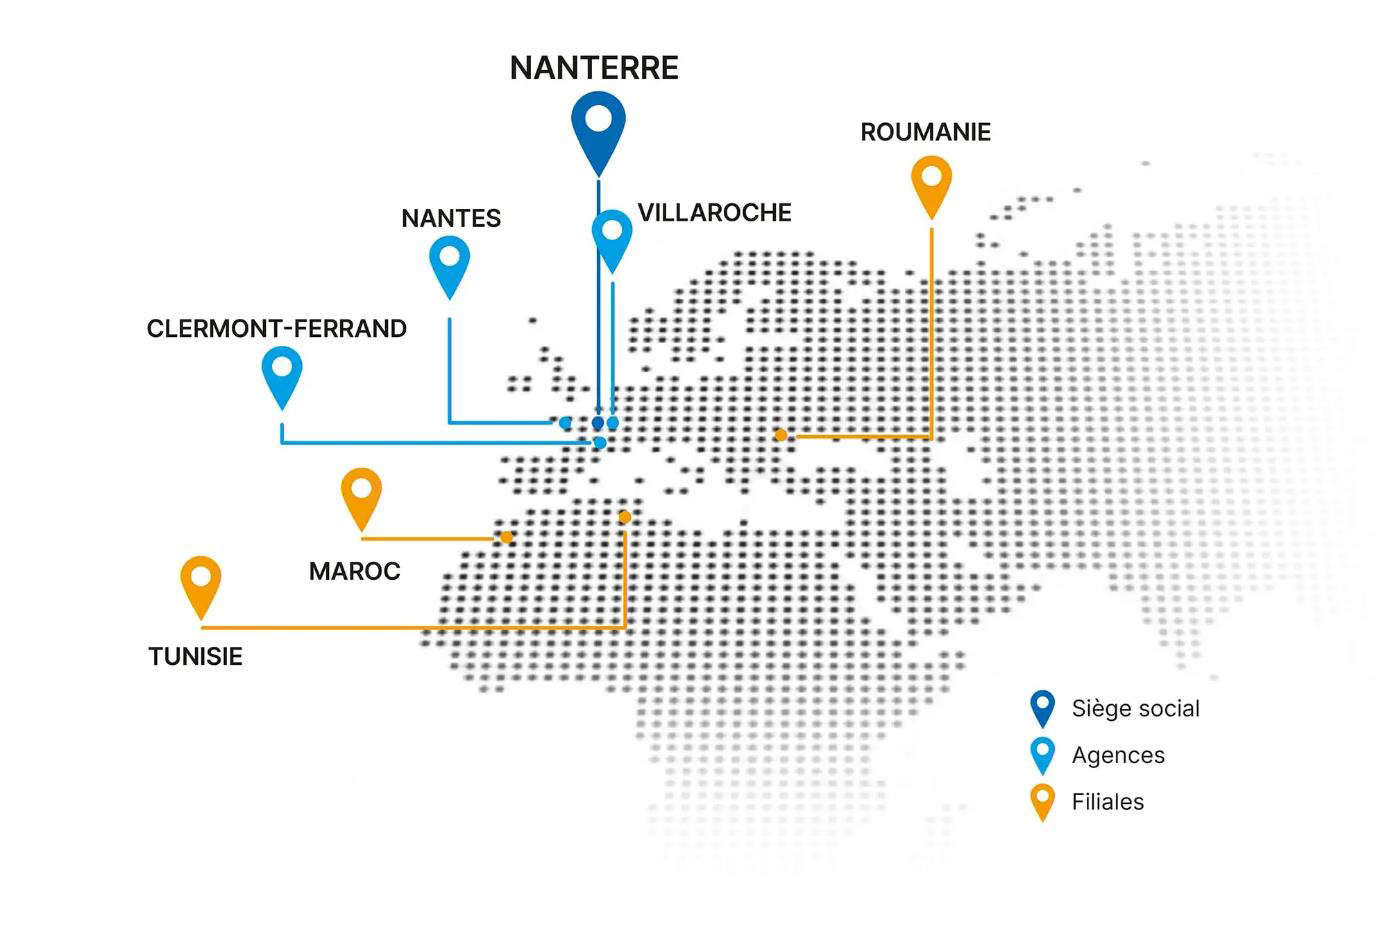
\includegraphics[width=1\linewidth]{Corps_rapport/sherpa.png}
    \captionof{figure}{Carte des agences de SHERPA Engineering dans le monde}
    \label{fig1}
\end{center}
$\ $\\
Elle est divisée en 3 Poles de direction:\\
\begin{itemize}
\renewcommand{\labelitemi}{$\bullet$}
    \item Direction Administrative et Financière
    \item Direction de l'Ingénierie
    \item Direction Stratégique\\
\end{itemize} 
Voici l'organigramme (\hyperref[fig2]{Figure 2}) de l'entreprise afin de mieux comprendre la structure.
\begin{center}
    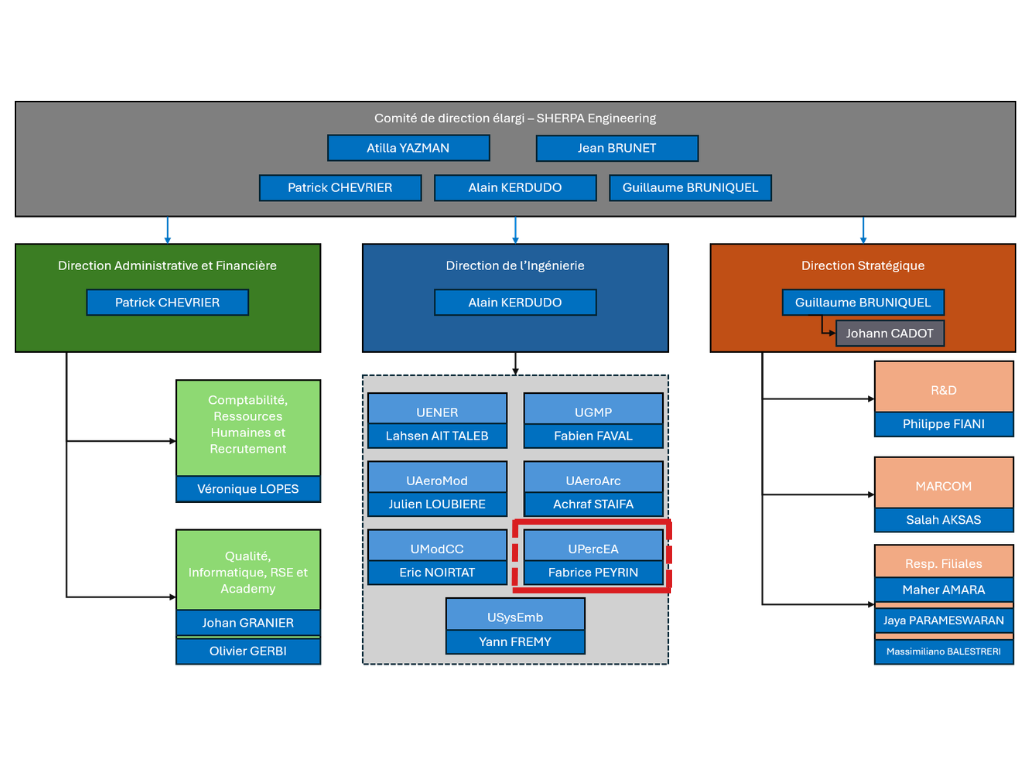
\includegraphics[width=1\linewidth]{Corps_rapport/Organigramme_SHERPA.png}
    \captionof{figure}{Organigramme de SHERPA Engineering}
    \label{fig2}
\end{center}
$\ $\\
\indent Au coeur de cette organisation, je fais partie de l'équipe UPercEA, dirigée par Fabrice PEYRIN. Cette équipe est partagée entre l'agence de Clermont-Ferrand et celle de Nantes. Mon tuteur de stage est Thomas Barbier, ingénieur en robotique spécialisé en vision artificielle.
